\begin{titre}[Fonctions de référence]

\Titre{La fonction Inverse}{4}
\end{titre}



\begin{CpsCol}
\textbf{Variations de fonctions}
\begin{description}
\item[$\square$] Connaitre la fonction Inverse : définition et courbes représentative.
\item[$\square$] Pour la fonction Inverse, résoudre graphiquement ou algébriquement une équation ou une inéquation du type $f(x) = k$, $f(x) < k$.
\item[$\square$] Étudier la parité d'une fonction dans des cas simples.
\end{description}
\end{CpsCol}




\begin{DefT}{Fonction Inverse}\index{Fonctions!Inverse}
La \textbf{fonction Inverse} $f$ est la fonction définie sur $\R^*$ par $f(x)=\frac{1}{x}$.
\end{DefT}


\begin{DefT}{Représentation graphique} \index{Fonction Inverse! Représentation graphique}\index{Hyperbole| see Fonction Inverse! Représentation graphique}
La \textbf{représentation graphique} de la fonction Inverse s'appelle une \textbf{hyperbole} et son équation est $y=\frac{1}{x}$. 
\end{DefT}



\begin{Pp}[Variations]
\begin{minipage}{0.48\linewidth}
La fonction Inverse est strictement décroissante sur $\R^*_-$ et strictement décroissante sur $\R^*_+$. 

L'hyperbole d'équation $y=\frac{1}{x}$ est symétrique par rapport à l'origine du repère.
\end{minipage}
\hfill
\begin{minipage}{0.48\linewidth}
\begin{tikzpicture}
\tkzTabInit[lgt=1,espcl=2]{ $x$ / 1,$f $ / 2}
{ $-\infty$ , $0$ ,$+\infty$}
\tkzTabVar{+/$0$ , -D+ /$ $/$ $ , -/$0$}
\end{tikzpicture}
\end{minipage}
\end{Pp}

\ROC

\mini{
\EPCB{1}{FR-6}{Raisonner.}
 
\EPCB{1}{FR-8}{Raisonner.}

\EPCC{1}{FR-11}{Représenter. Raisonner.}
}{
\EPCB{1}{FR-12}{Représenter. Raisonner.}

\EPCB{1}{FR-19}{Raisonner. Calculer.}
}


\mini{
%\EPCB{1}{FR-13}{Représenter. Raisonner. Calculer}

\EPCB{1}{FR-14}{Représenter. Raisonner. Calculer}

%\EPCB{1}{FR-21}{Représenter. Raisonner. Calculer}
\EPCB{1}{FR-18}{Représenter. Raisonner. Calculer}
}{


\EPCC{1}{FR-16}{Représenter. Raisonner. Calculer}

\EPCC{1}{FR-20}{Représenter. Raisonner. Calculer}
}





